\scanpage{123}
% archive sheet number: 122
\diagram{\begin{tikzcd}[ampersand replacement=\&,column sep=small,row sep=small]
 \unsure{\zeta_1|\xi_1}\arrow[d,maps to]\&\zeta_2\arrow[d,maps to]\&\zeta_3\arrow[d,maps to]\&{}\in k\&\infty\arrow[dl,maps to,out=270,in=75]\\
 0\&1\&\infty\&t
\end{tikzcd}}
\[
 \left\{\begin{aligned}&\zeta_1,1\\&\zeta_2,1\\&\zeta_3,1\end{aligned}\right.
\]
\figure{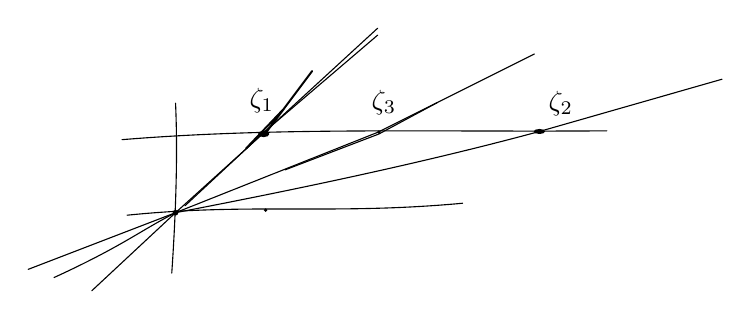
\begin{tikzpicture}[x=.008cm,y=.008cm,line cap=round,line join=round]
 \draw (-85,116) .. controls (160,136) and (398,128) .. (685,130);
 \draw (-77,-4) .. controls (120,16) and (250,-4) .. (456,15);
 \draw (-6,-96) .. controls (2,22) and (3,107) .. (0,174);
 \draw (-133,-124) -- (0,0) -- (137,124) -- (321,293);
 \draw[thin] (15,11) -- (143,130) -- (321,282);
 \draw[line width=.7pt] (112,102) -- (173,166) -- (142,125) -- (217,225);
 \draw (-193,-103) .. controls (-86,-54) and (-55,-28) .. (0,0) -- (322,128) -- (570,252);
 \draw[thin] (174,68) -- (323,125) -- (416,175);
 \draw (-234,-90) -- (0,0) .. controls (166,32) and (378,75) .. (578,129) -- (868,212);
 \fill (0,0) circle[radius=.036cm]; \fill (140,125) ellipse[x radius=.072cm,y radius=.040cm]; \fill (323,128) circle[radius=.024cm];
 \fill (578,129) ellipse[x radius=.072cm,y radius=.032cm]; \fill (143,4) circle[radius=.024cm];
 \node[above] at (137,143) {$\zeta_1$}; \node[above] at (331,140) {$\zeta_3$}; \node[above] at (612,138) {$\zeta_2$};
\end{tikzpicture}}
\[
 \begin{aligned}&\lambda_1\zeta_1,\lambda_1\\&\lambda_2\zeta_2,\lambda_2\\&\lambda_3\zeta_3,\lambda_3\end{aligned}
 \qquad\left[\begin{aligned}
 &\sum\lambda_i=0\\ &\sum\lambda_i\zeta_i=0\qquad \zeta_1,\zeta_2,\zeta_3\ \text{tous distinct}\\
 &\text{Cela détermine }(\lambda_i)\text{ mod }\inserted{\text{mult. par}}\text{ scalaire inv.}
 \end{aligned}\right.
\]
\[
 \begin{array}{rcl@{\qquad}|l}
 &&&\multicolumn{1}{l}{\unsure{01|O1}}\\
 \lambda_1&=&\zeta_{\underline2}-\zeta_{\underline3}&\zeta_1\\
 \lambda_2&=&\zeta_{\underline3}-\zeta_{\underline1}&\zeta_2\\
 \lambda_3&=&\zeta_{\underline1}-\zeta_{\underline2}&\zeta_3
 \end{array}
 \qquad\left\{\deleted{\Bigg\{}
 \begin{aligned}
 \unsure{e'_2|e_2}-e_3&=((\zeta_2-\zeta_3)\zeta_1,\zeta_2-\zeta_3)\\
 e_3-e_1&=((\zeta_3-\zeta_1)\zeta_2,\zeta_3-\zeta_1)\\
 e_1-e_2&=((\zeta_1-\zeta_2)\zeta_3,\zeta_1-\zeta_2)
 \end{aligned}\right.
\]
\[
 \deleted{\unsure{e_2}}\quad \deleted{f_1\longrightarrow}\qquad
 \deleted{(\zeta_1,1)\unsure{1|\mapstochar}\longrightarrow}\quad\zeta_1f_1+
\]
